% htts://pxl-digital.pxl.be/page/studentenreis-2020-berlijn2

In de opleiding hoorde ook een deel over internationalisering uitgevoerd te worden. Hierdoor was er onder andere de mogelijkheid om op studiereis te gaan met medestudenten. Ik heb deze kans gegrepen en heb gekozen voor de studiereis naar Berlijn. Je kon kiezen tussen verschillende reizen. Er was er namelijk één naar Amsterdam en twee naar Berlijn. Die naar Amsterdam heb ik niet gekozen omdat ik de stad reeds vaker bezocht had en omdat het belangrijkste onderwerp van deze reis Cisco was, hetgeen mij niet echt aansprak. Bijgevolg bleven nog twee opties over waarbij ik het bezichtigen van de universiteit verkoos boven deelname aan de makathon.

De reis startte uiteraard met een lange busrit. Hier leerden we de groep wat beter kennen. Eenmaal aangekomen konden we inchecken in de kamer van het hotel en hadden we de rest van de avond nog vrij om Berlijn te gaan verkennen of om uit te rusten voor de drukke dagen die we tegemoet gingen komen.

Tijdens de eerste echte dag in Berlijn werden we opgesplitst in twee groepen om afwisselend de geplande activiteiten uit te voeren. Zo vertrok de ene groep naar de Stasi\hyp{}gevangenis Hohensch\"onhausen en de andere naar de Tempelhof luchthaven. In de namiddag wisselden de groepen van activiteit. In de gevangenis kregen we een rondleiding van een ex\hyp{}gevangene. Dit was zowel een voor\hyp{} als een nadeel. De spreker zijn Engels was niet erg goed waardoor hij initieel zeer moeilijk te verstaan was. Achteraf kon hij echter op een fascinerende manier zijn ervaringen en gevoelens delen met de groep, hetgeen zeker een meerwaarde vormde. Hij had een zeer fascinerende houding ten opzichte van de gevangenis en de bewakers van toen.

Daarna kregen we een rondleiding in de luchthaven, wat vroeger één van de grootste gebouwen van Europa was. Aangezien het een gigantisch gebouw omvatte, hebben we hier veel moeten wandelen, al was dit zeker en vast de moeite. De luchthaven was, toen wij hem bezochten, volledig leeg en verlaten, op een aantal ruimtes na. Dankzij de goede uitleg en aanvullende attributen kregen we toch een goed idee over hoe de luchthaven functioneerde gedurende zijn hoogtepunt en waarom dat hij zo goed bewaard is gebleven gedurende de oorlog. Ook werd aan ons verduidelijkt wat zijn huidige functie is en wat men in de toekomst nog ermee plande te doen.

De volgende dag was een toeristische rondleiding gepland in Berlijn. Zo reden we eerst met de bus door Berlijn en gaf een gids uitleg over monumenten en straten waar we langs of door reden. Na deze busrit gingen we te voet verder met de gids. Zo bezochten we bekende monumenten als de Berlijnse Muur, Checkpoint Charlie, Potsdamer Platz, de Berliner Dom, het Holocaust monument en nog veel meer. De gids gaf een goede uitleg over het verleden van deze monumenten maar ook de huidige betekenis en waarde ervan. Normaal gesproken ben ik geen grote voorstand van een rondleiding met een gids, maar door deze gids ben ik zeer aangenaam verrast omdat we veel hebben kunnen bezichtigen met een interessante uitleg en op korte tijd.

\begin{figure}[!h]
  \centering
  \begin{subfigure}[h]{0.48\textwidth}
    \centering
    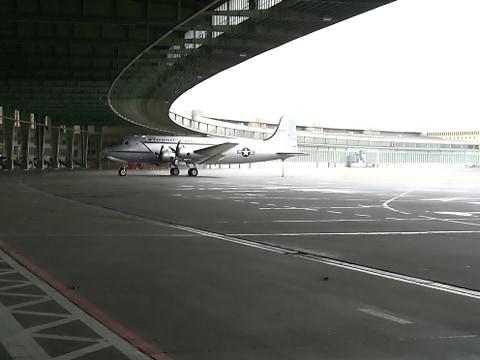
\includegraphics[width=0.85\linewidth]{images/berlijn/tempelhof.jpg}
    \caption{Tempelhof luchthaven}
  \end{subfigure}
  \begin{subfigure}[h]{0.48\textwidth}
    \centering
    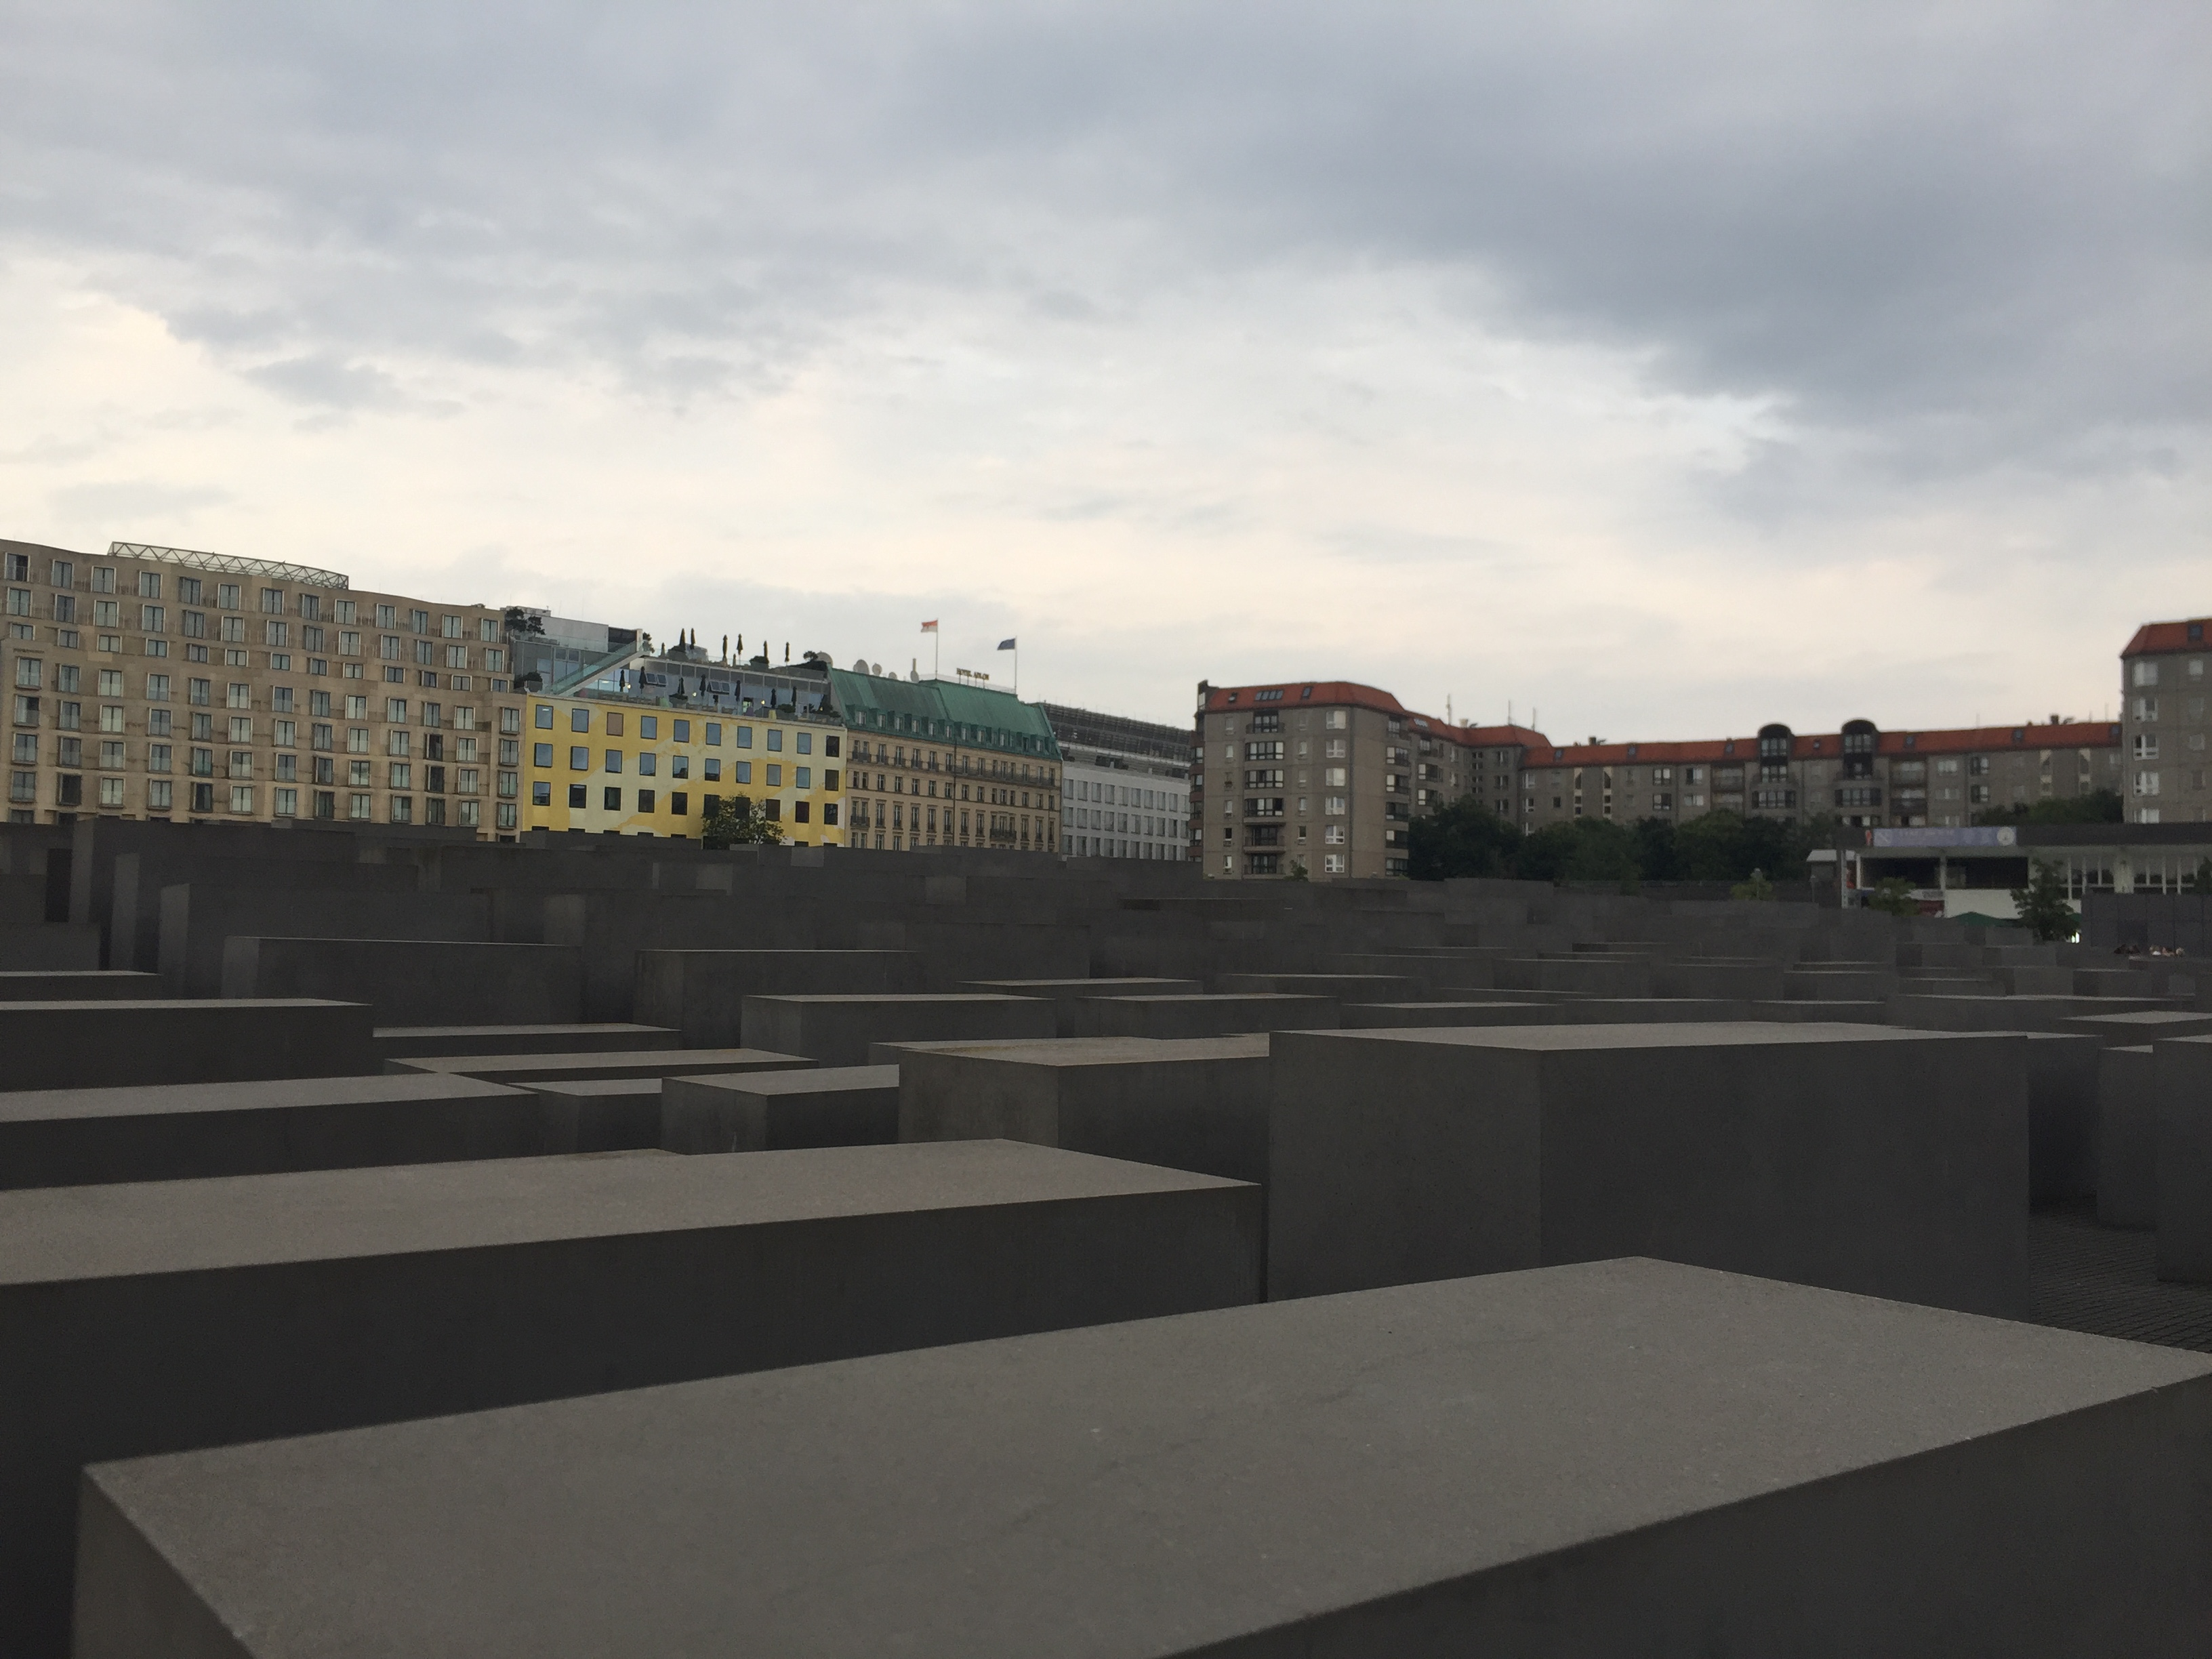
\includegraphics[width=0.85\linewidth]{images/berlijn/holocaust_monument.jpg}
    \caption{Holocaust monument}
  \end{subfigure}
\end{figure}

De laatste dag in Berlijn zouden we normaal naar de Technische Universit"at Berlin gaan en daar een seminarie volgen rond Future Security Lab, maar dit is niet door kunnen gaan omwille van een voor ons onbekende reden. Na de middag kregen we op diezelfde locatie normaalgezien ook een verrassingsseminarie, maar bijgevolg hebben we dit seminarie ook niet kunnen volgen. Omdat onze begeleiders deze late annulering niet hadden voorzien, mochten we de dag zelf inplannen. In groep zijn we Berlijn nog wat verder gaan verkennen en hebben we genoten van de stad. Ook hebben we kunnen uitrusten van de vermoeide afgelopen dagen. Na een korte nacht, zijn we uitgecheckt uit het hotel, hebben we ontbeten en zijn we de bus opgestapt richting Hasselt.

De studiereis was zeker geslaagd voor mij. Desondanks vond ik het jammer dat we niet naar de universiteit zijn kunnen gaan. Ik heb mijn medestudenten zeker beter leren kennen en nieuwe vrienden gemaakt, hetgeen ik vooraf niet had verwacht. De leuke groepssfeer maakte deze reis voor mij een unieke ervaring.

Op de onvoorziene omstandigheden na, zou ik de reis zeker opnieuw doen en aanraden aan de andere studenten. Het enige dat naar mijn mening minder aangenaam was, zijn de lange busritten, maar uiteraard horen ook zij erbij. Het was een vermoeiende reis door de relatief korte nachten en lange dagen, maar ook dit was het waard.

Ik heb deze opdracht opgenomen in mijn portfolio omdat deze studiereis een grote indruk heeft nagelaten op mij en het een groot deel uitmaakte van mijn derde en belangrijkste jaar op Hogeschool PXL. Ook omdat op gebied van mijn medestudenten leren kennen, dit toch een van de meest impactvolle elementen is en het plezier maken met elkaar.

\begin{figure}[!h]
  \centering
  \begin{subfigure}[h]{0.48\textwidth}
    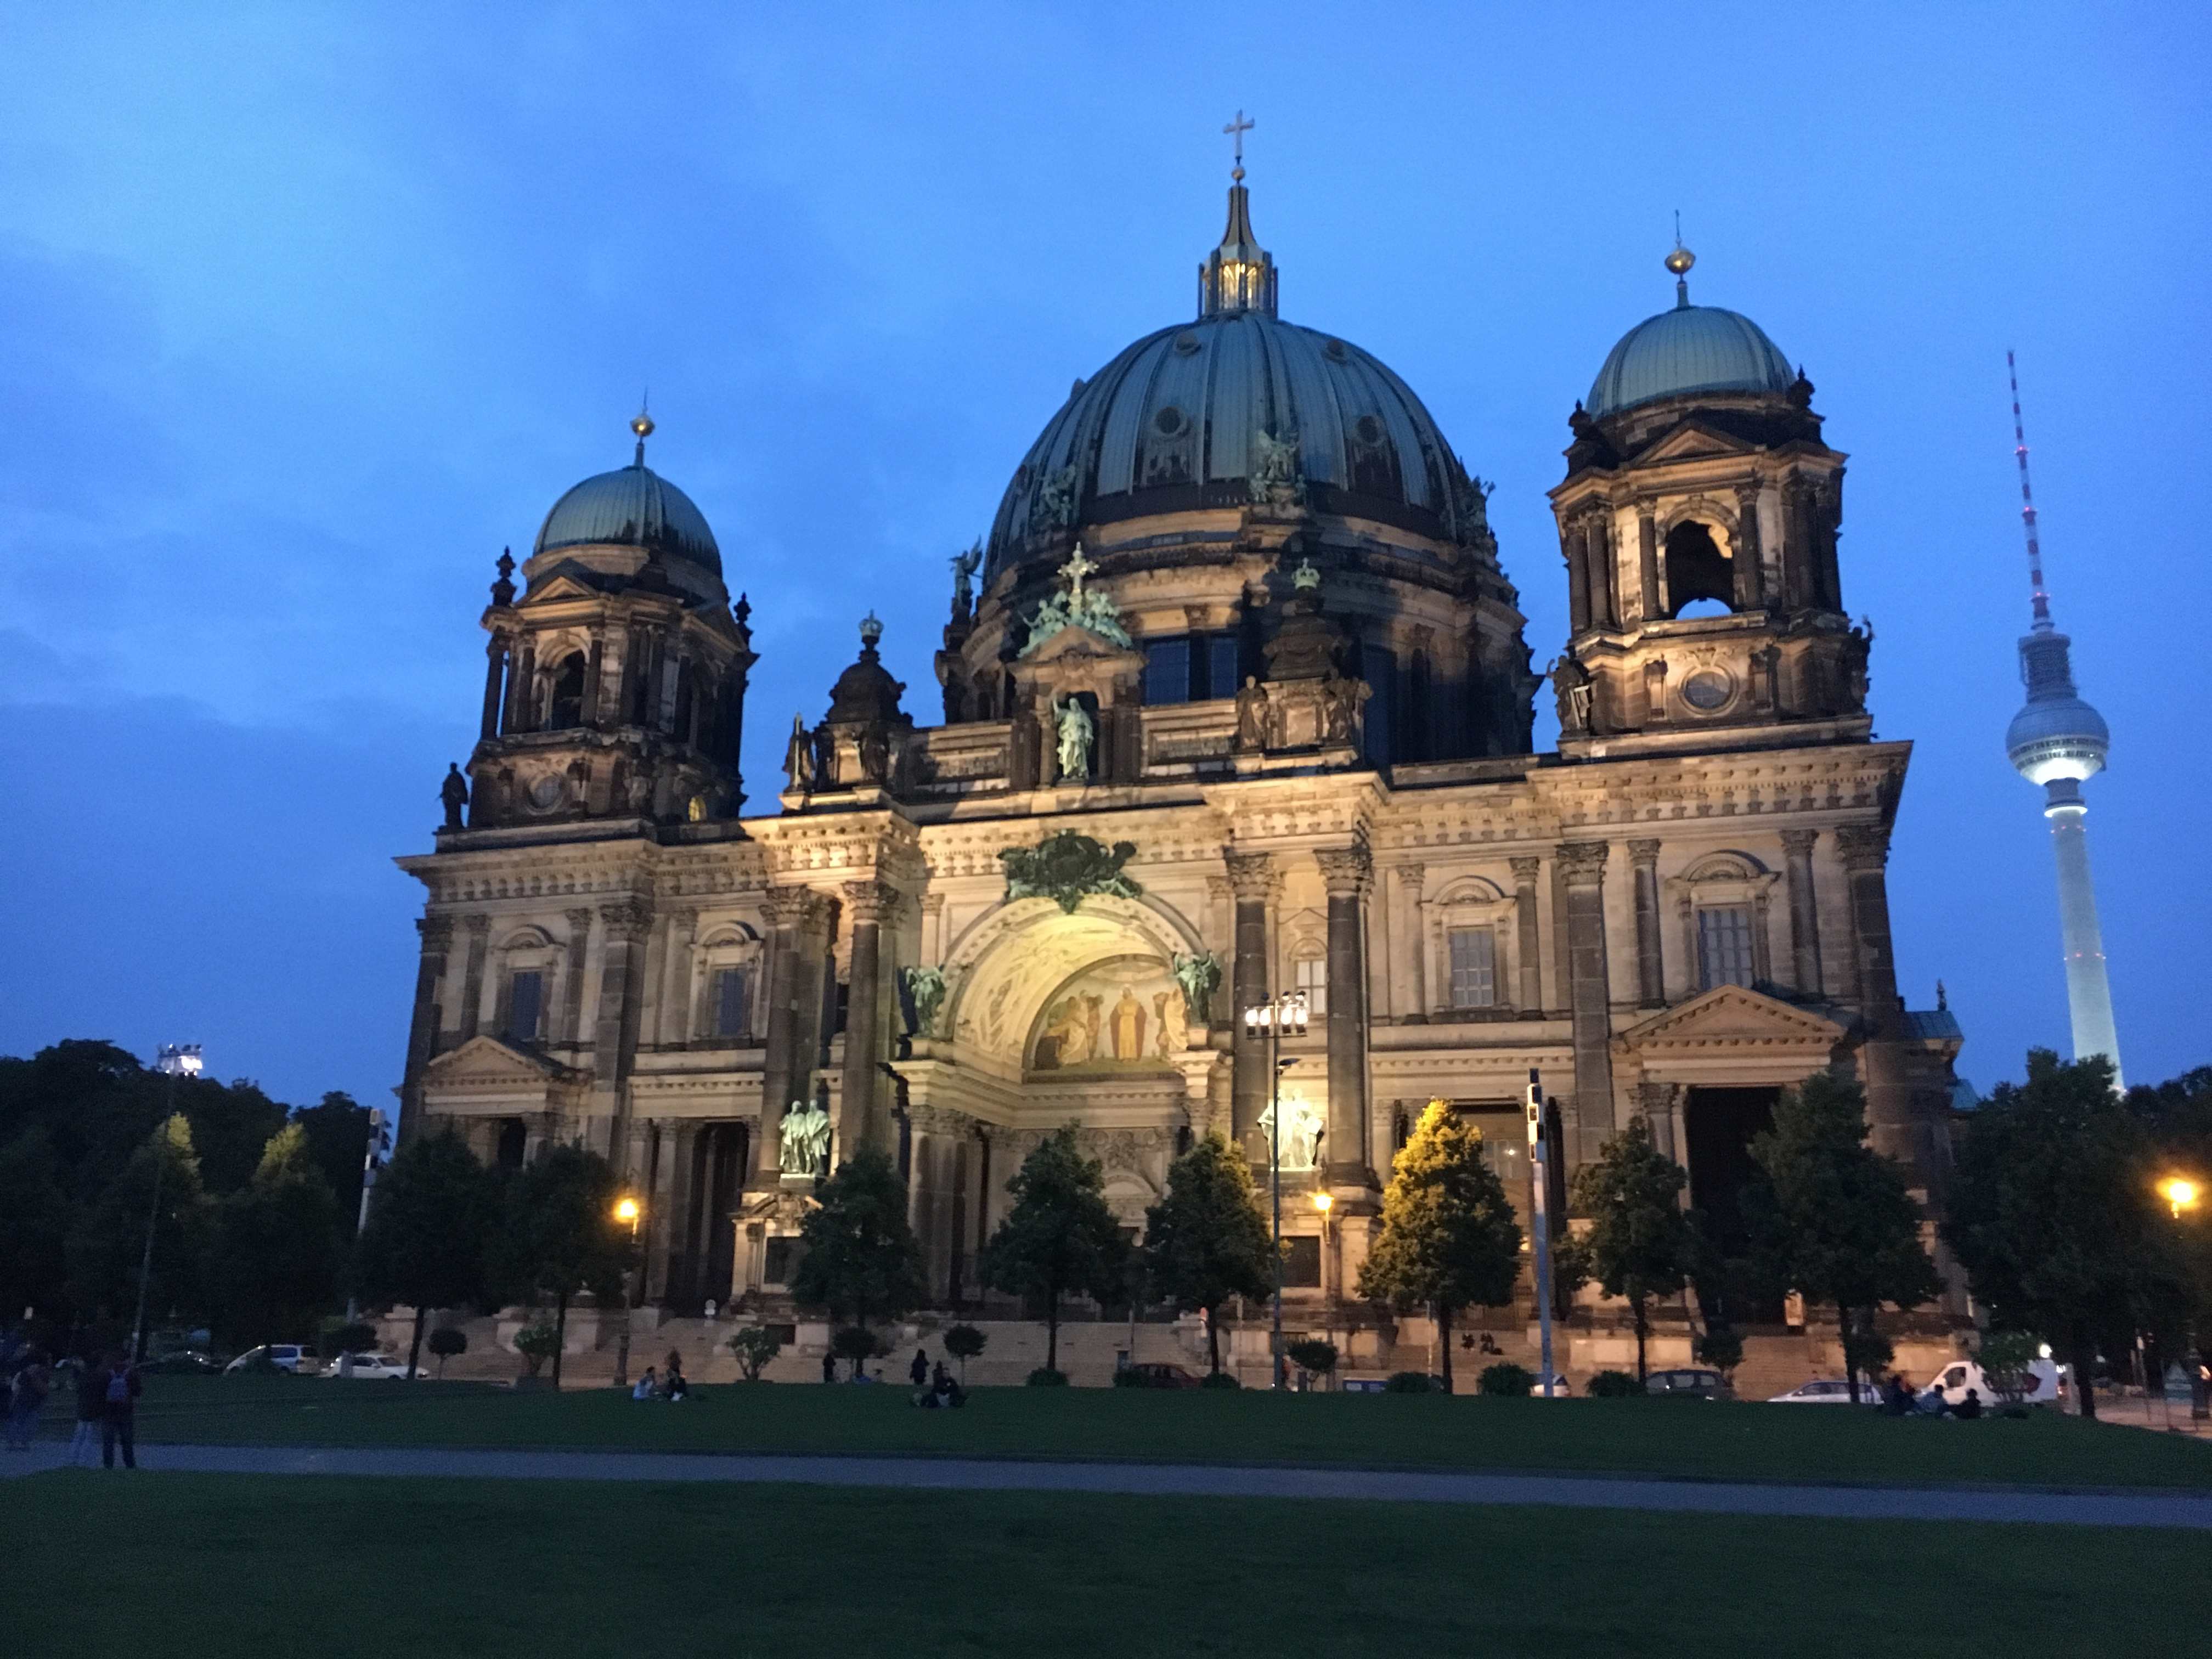
\includegraphics[width=\linewidth]{images/berlijn/berliner_dom.jpg}
    \caption{Berliner Dom}
  \end{subfigure}
  \begin{subfigure}[h]{0.48\textwidth}
    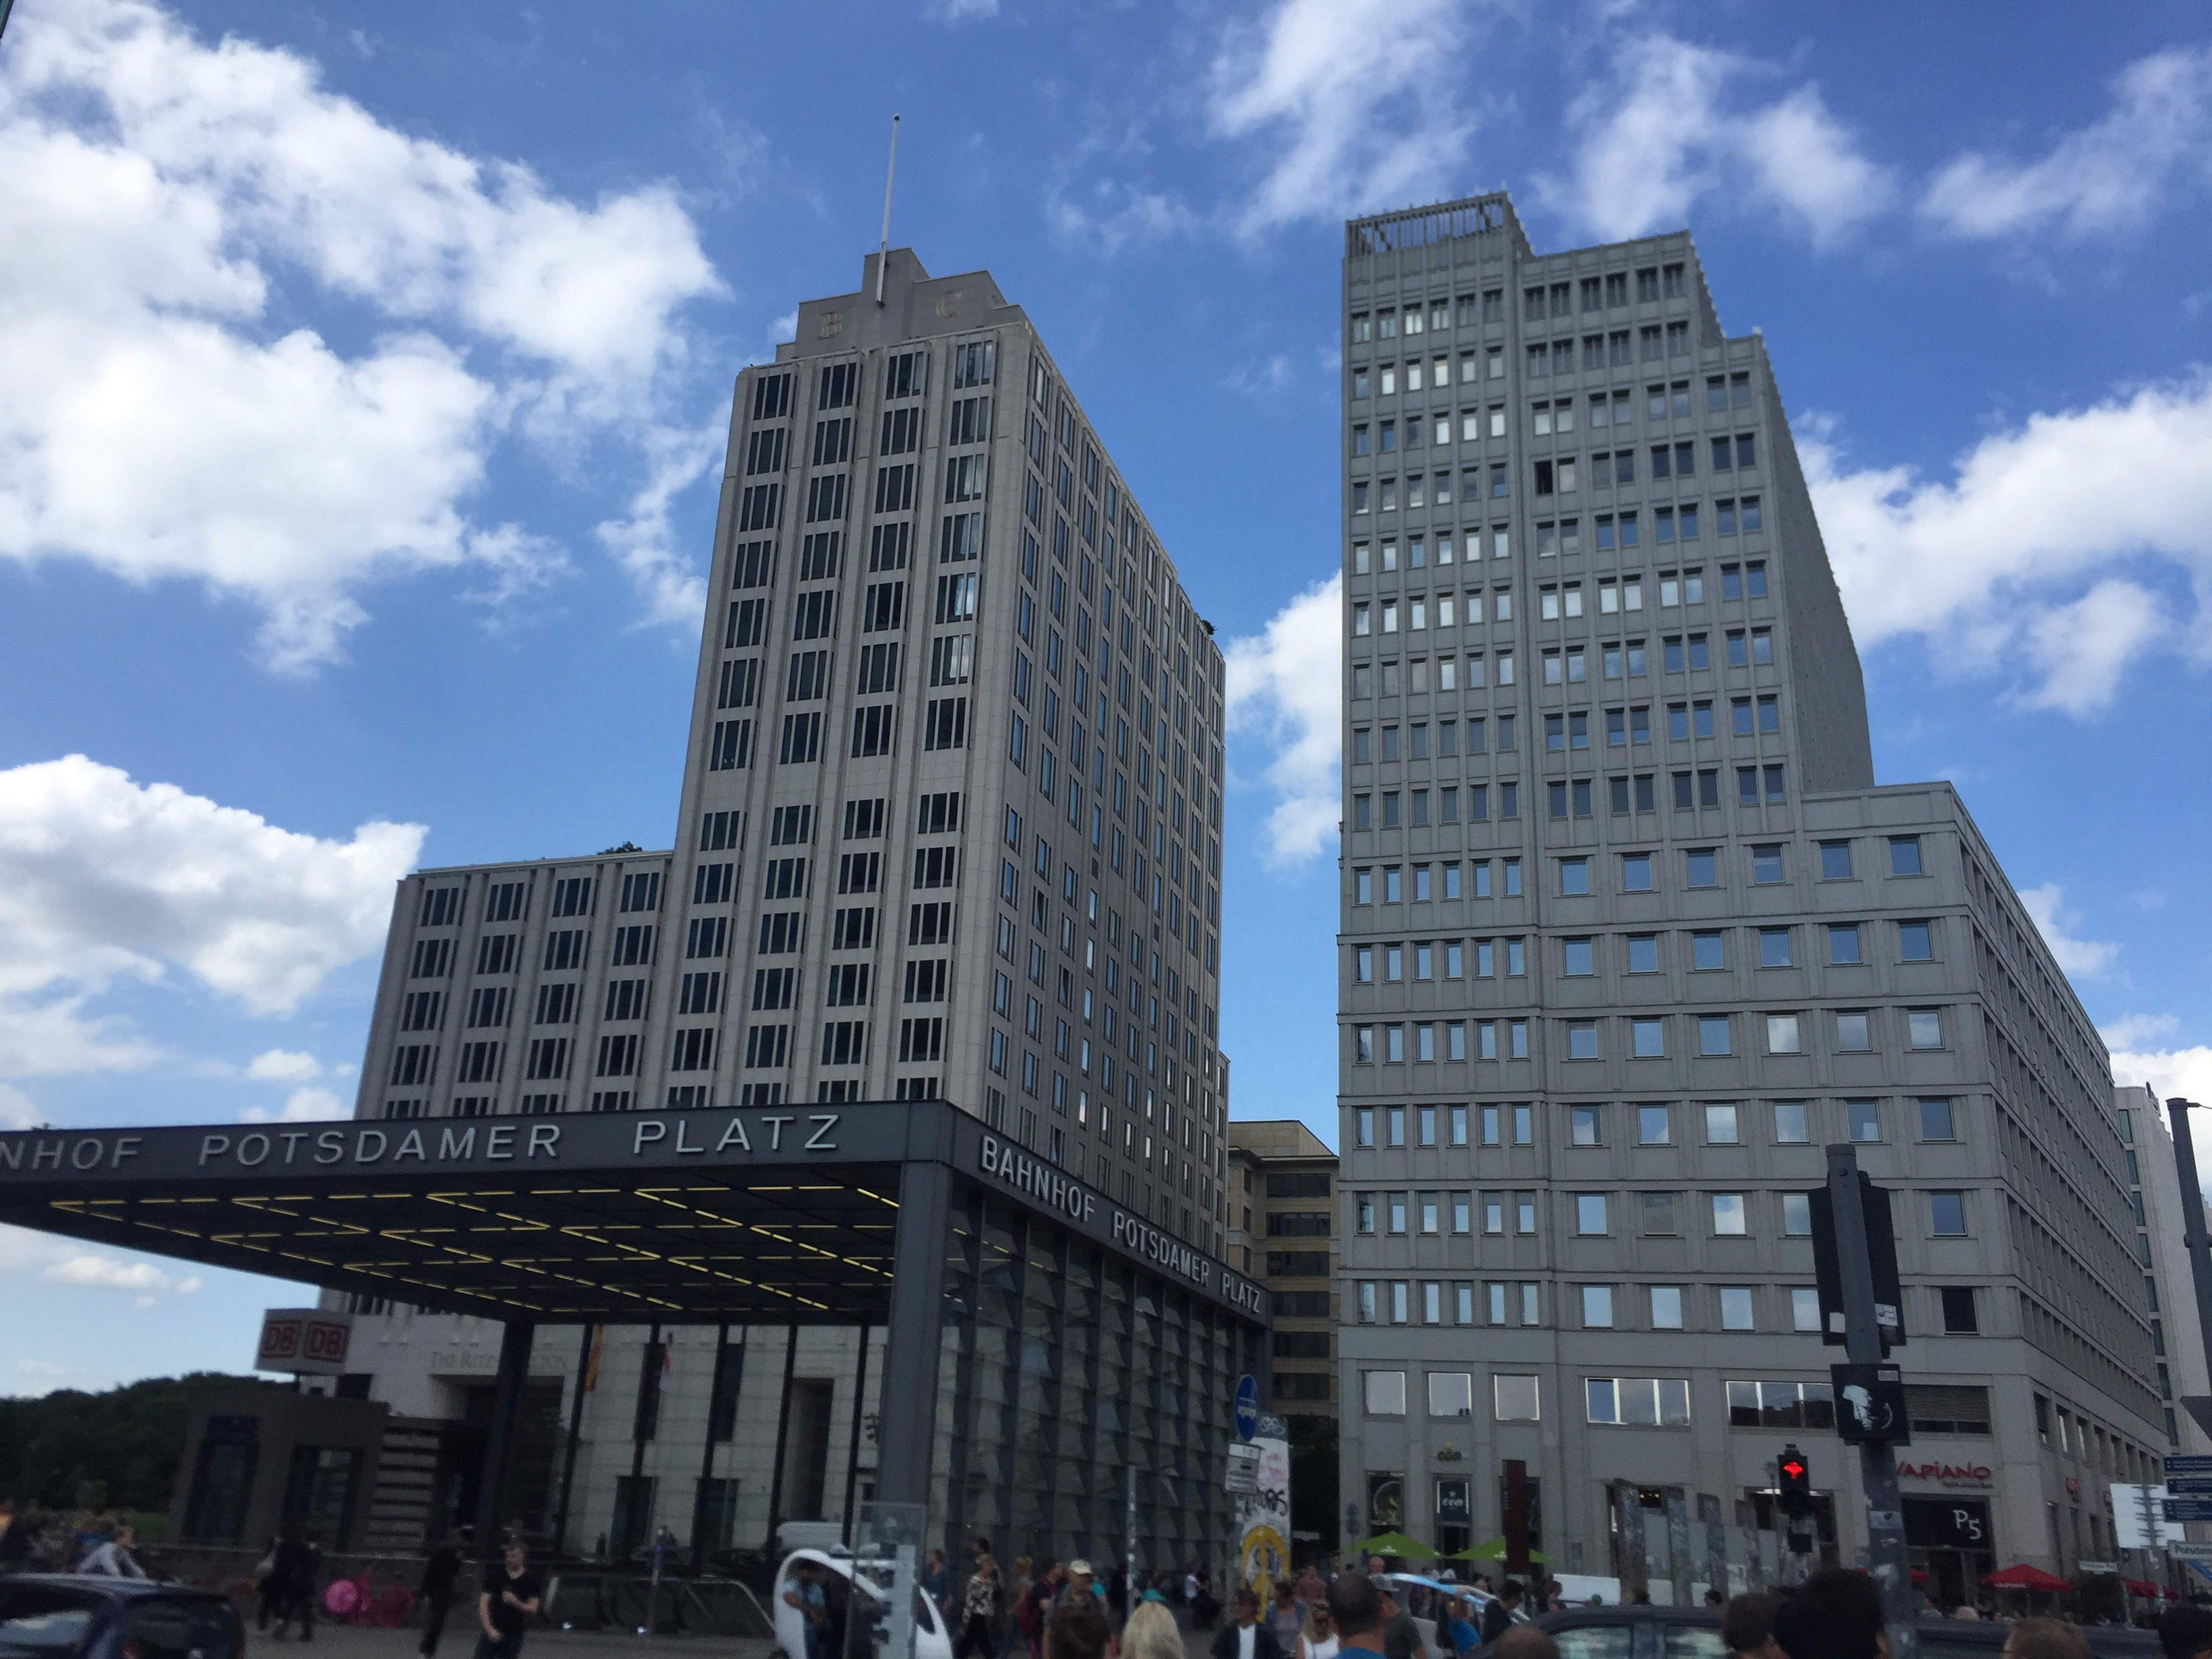
\includegraphics[width=\linewidth]{images/berlijn/potsdamer_platz.jpg}
    \caption{Portzdamer Platz}
  \end{subfigure}
  \begin{subfigure}[h]{0.48\textwidth}
    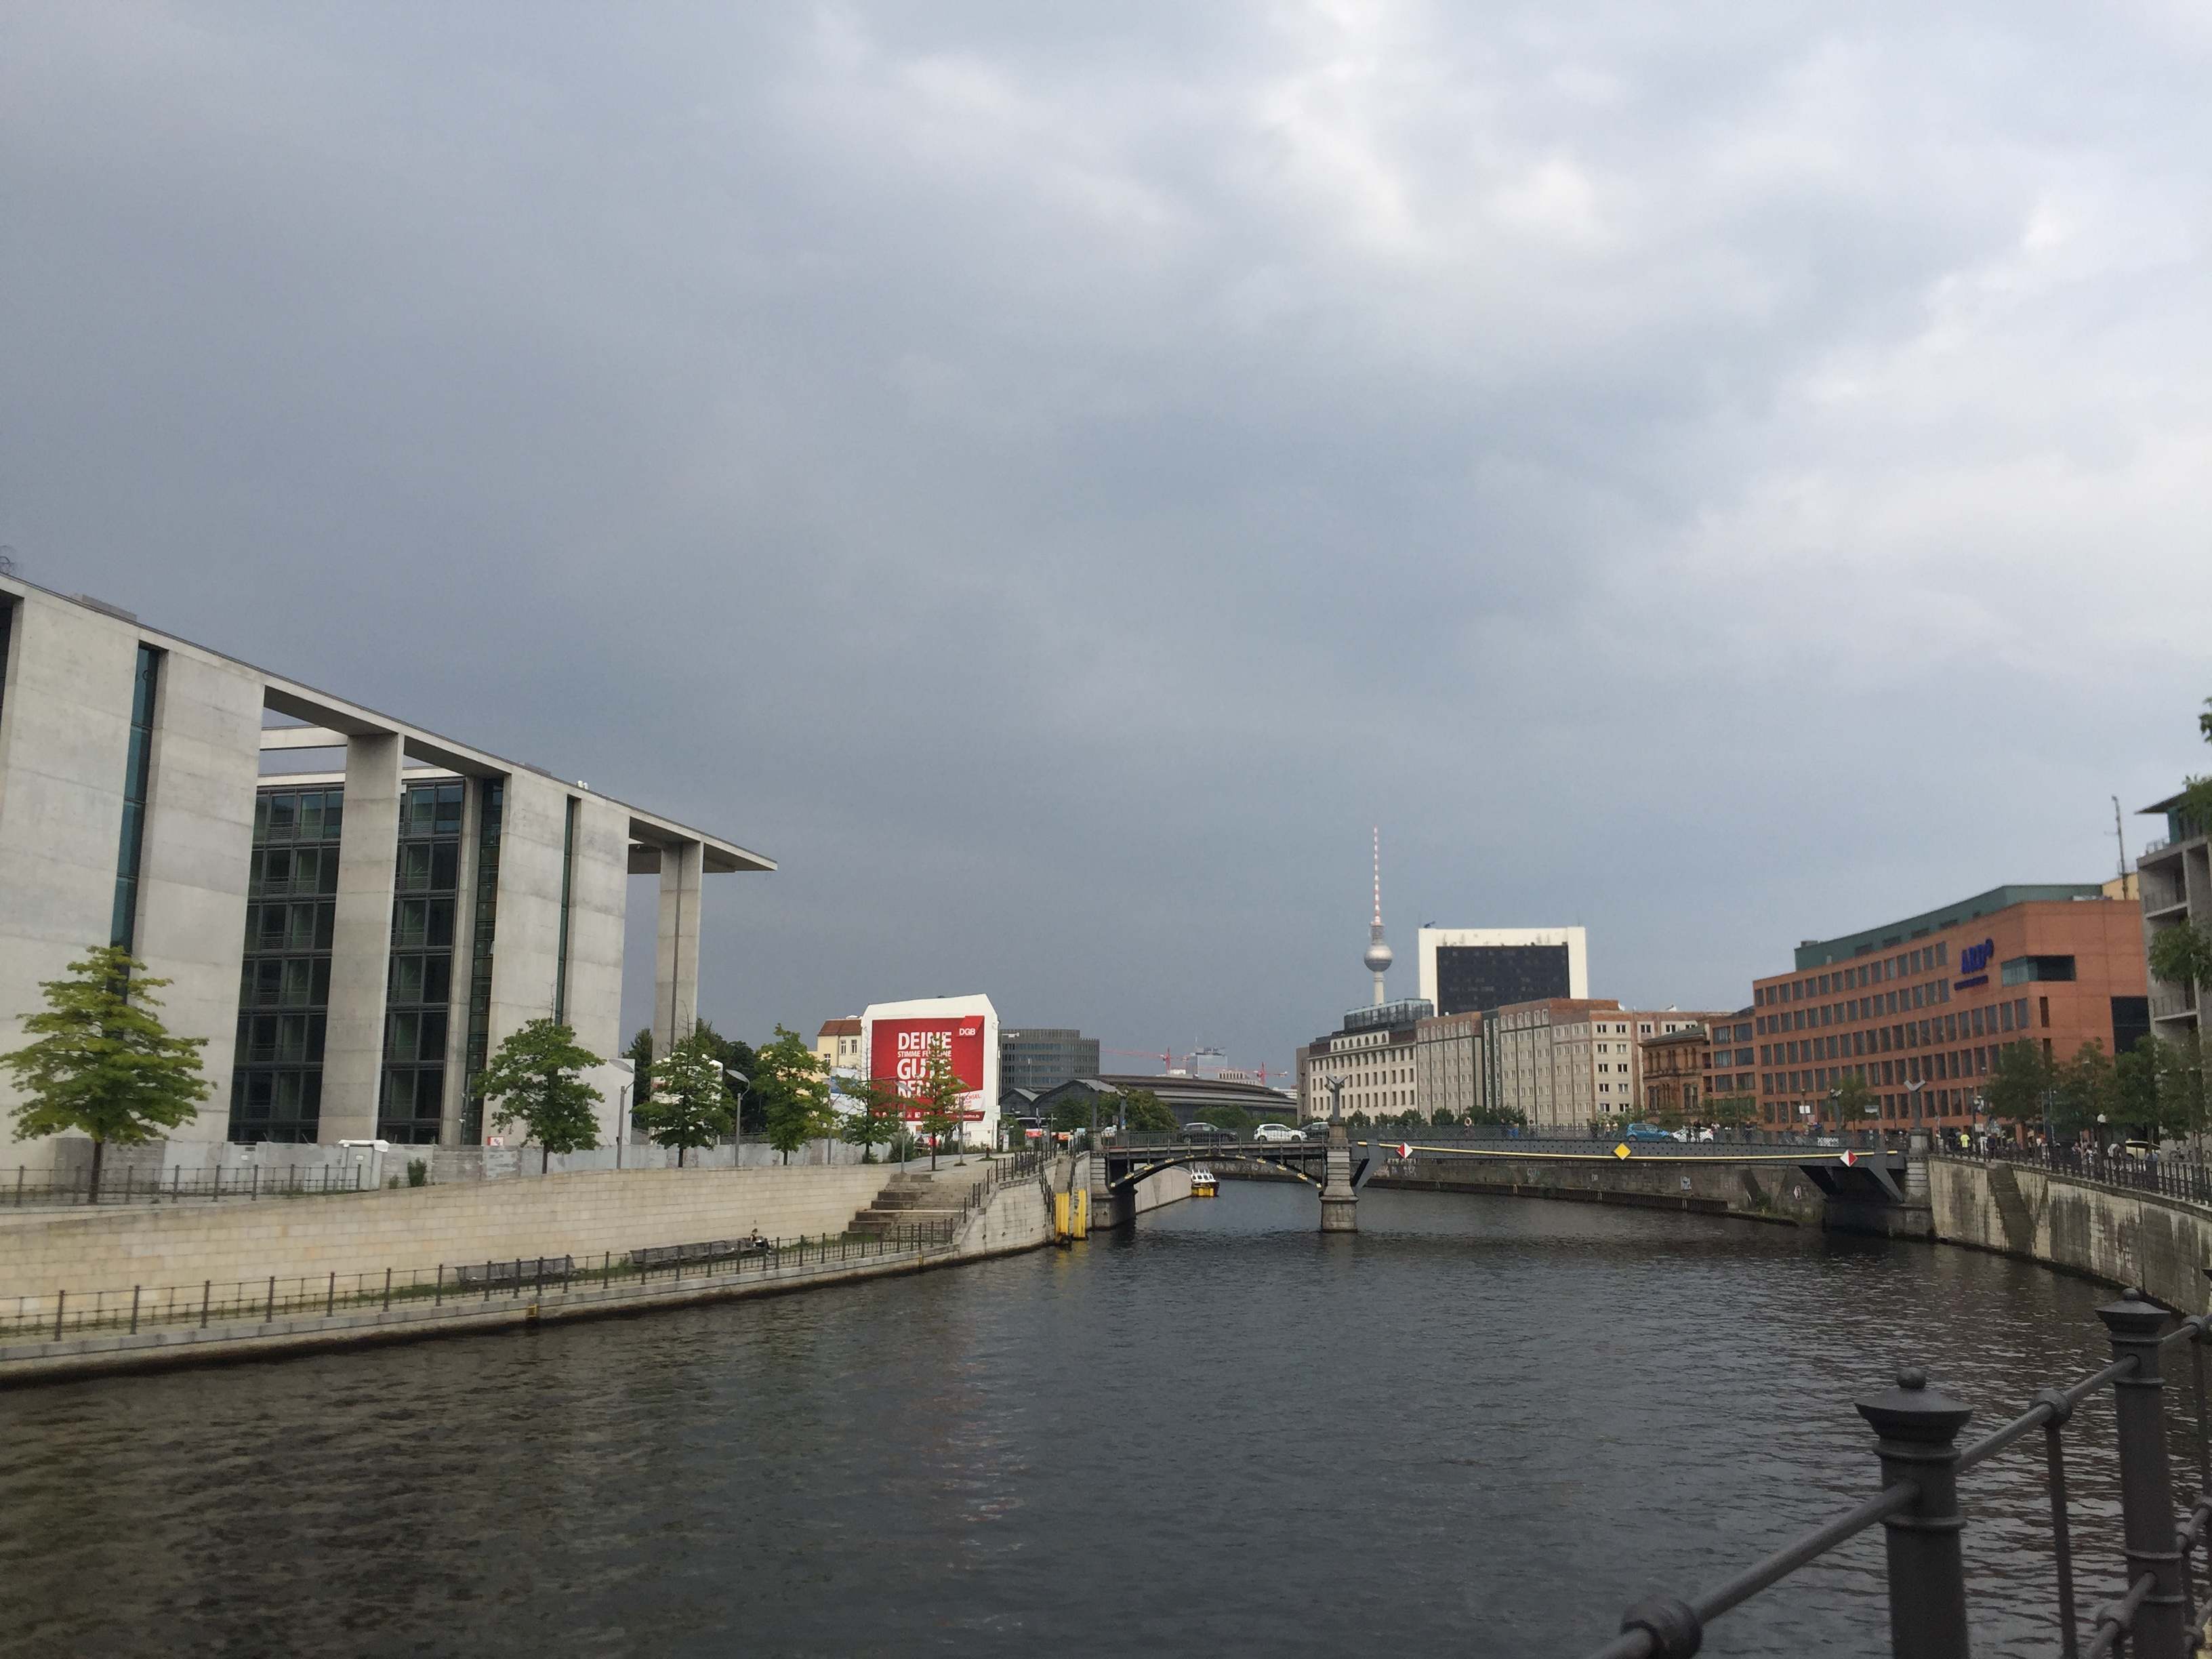
\includegraphics[width=\linewidth]{images/berlijn/uitzicht_reichstag.jpg}
    \caption{Uitzicht vanaf Reichstag}
  \end{subfigure}
  \begin{subfigure}[h]{0.48\textwidth}
    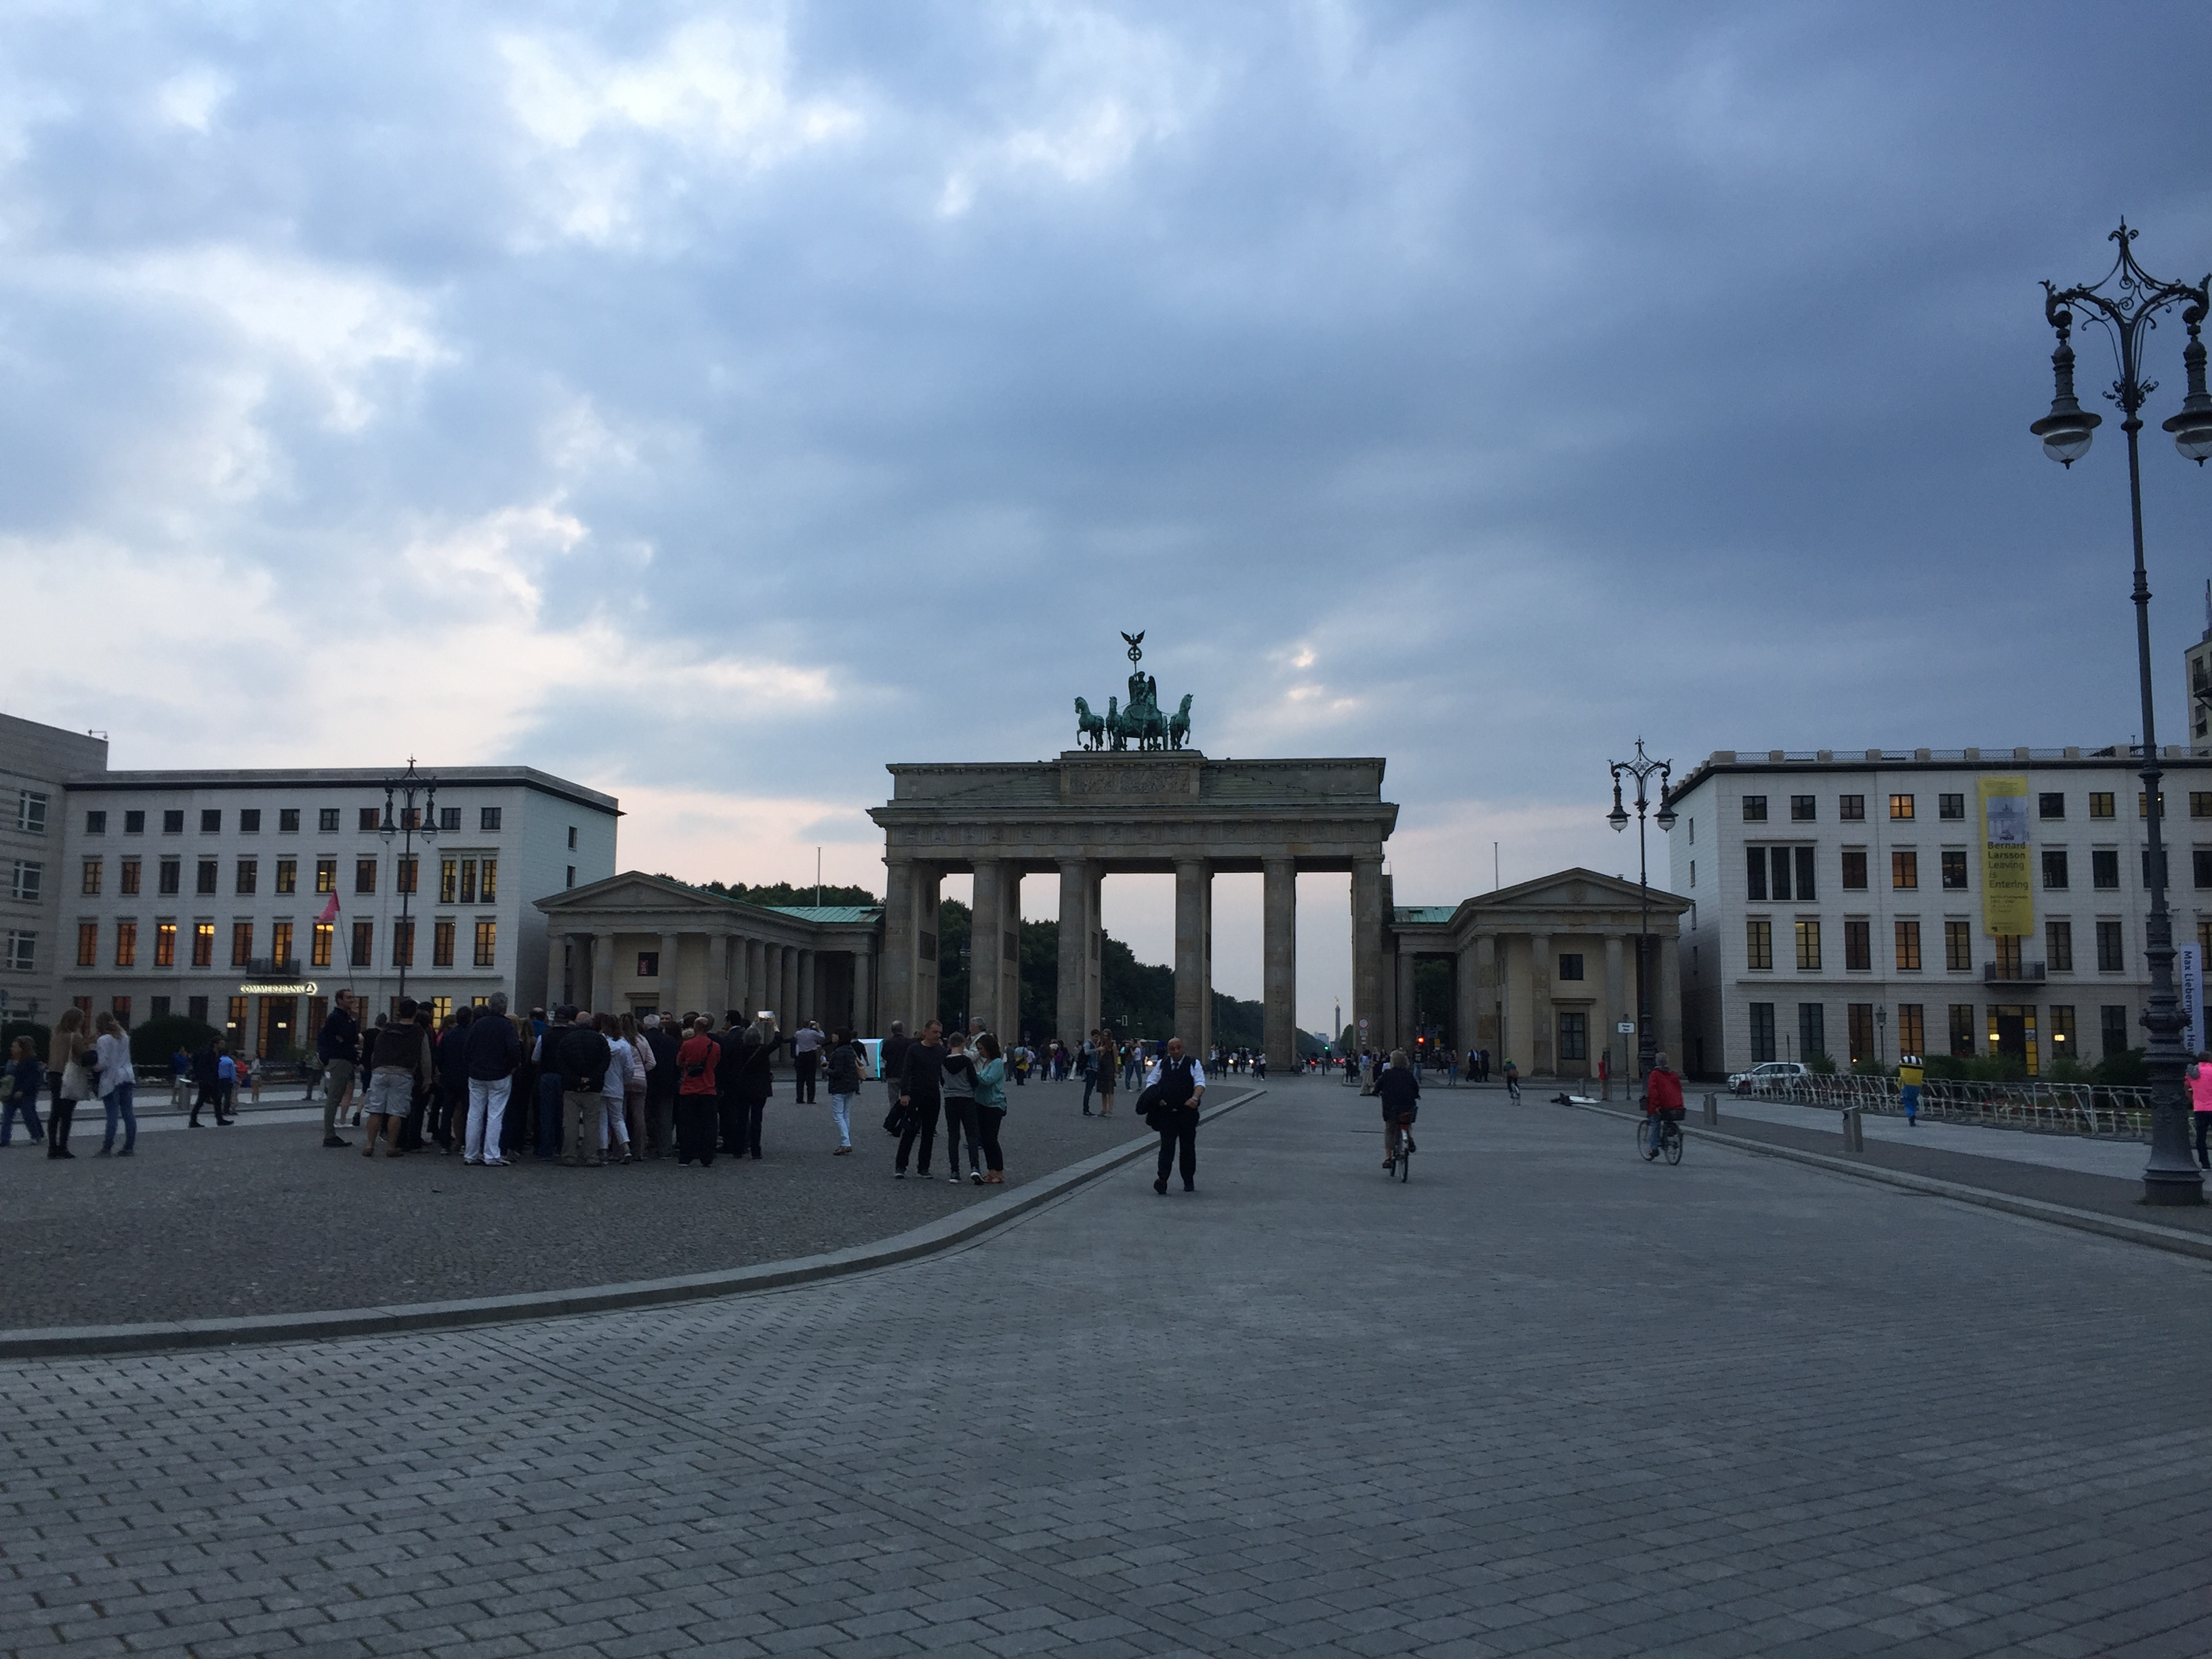
\includegraphics[width=\linewidth]{images/berlijn/brandenburger_tor.jpg}
    \caption{Brandenburger Tor}
  \end{subfigure}
\end{figure}